\section{Sucesión de Mayer-Vietoris}

Una familia de grupos abelianos $\{A_n:n\in \N\}$ y morfismos $\alpha_n: A_n\to A_{n-1}$ constituye una $\textbf{sucesión exacta}$ si para todo $n\in\N$ se cumple $\Ker(\alpha_{n})=\im(\alpha_{n+1})$.

\begin{obs}

La inclusión $\im(\alpha_{n+1})\subset\Ker(\alpha_{n})$ nos dice que $\alpha_{n+1}\circ\alpha_{n}\equiv 0$, es decir, los $\alpha_n$ forman un complejo de cadenas. 

La otra inclusión, $\im(\alpha_{n+1})\supset\Ker(\alpha_{n})$, nos dice que los grupos de homología asociados a este complejo de cadenas son triviales.

En general, podemos interpretar la sucesión de grupos de homología asociados a un complejo de cadenas como un indicador de qué tan cerca está el complejo de ser una sucesión exacta.

\end{obs}

La existencia de la sucesión de Mayer-Vietoris para espacios topológicos va a surgir del siguiente hecho algebraico:

\begin{lema}{Lema de la serpiente}

	Sea $$0\rightarrow A\xrightarrow{f} B\xrightarrow{g} C\rightarrow 0$$ una sucesión exacta corta entre complejos de cadena. Entonces, para cada $n\in\Z$ existe un homomorfismo de grupos $$\delta_* :H_{n+1}(C)\rightarrow H_n(A)$$ tal que la siguiente sucesión es exacta:

	\begin{figure}[h!]
    	\centering
    	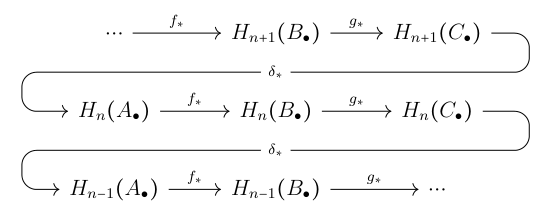
\includegraphics[width=0.5\linewidth]{img mono/mayer vietoris/serpiente.png}
    	\caption{tengo que aprender a hacer esto en tikz}
    	\label{serpiente}
	\end{figure}

\end{lema}

Dentro de un espacio topológico consideramos dos subespacios $A$ y $B$, y sea $X=\mathring{A}\cup\mathring{B}$. Definimos $C_n(A+B)$ el complejo de cadenas dado por la suma formal de las cadenas en $A$ y $B$. El mapa borde $\partial:C_{n}(X)\to C_{n-1}(X)$ manda elementos de $C_n(A+B)$ en elementos de $C_{n-1}(A+B)$, entonces los $C_n(A+B)$ forman un complejo de cadenas.

\[\begin{tikzcd}
	\dots & {C_n(A+B)} & {C_{n-1}(A+B)} & \dots \\
	\dots & {C_n(X)} & {C_{n-1}(X)} & \dots
	\arrow[from=1-1, to=1-2]
	\arrow[from=1-2, to=1-3]
	\arrow["i", hook, from=1-2, to=2-2]
	\arrow[from=1-3, to=1-4]
	\arrow["i", hook, from=1-3, to=2-3]
	\arrow[from=2-1, to=2-2]
	\arrow[from=2-2, to=2-3]
	\arrow[from=2-3, to=2-4]
\end{tikzcd}\]

$\textbf{Afirmación:}$ Las inclusiones $C_n(A+B)\hookrightarrow C_n(X)$ inducen isomorfismos en los grupos de homología. 

$$H_n(X)\simeq H_n(A+B)$$

\comm{falta probar esto}

Definiendo $\psi(x)=(x,-x)$, $\phi(x,y)=x+y$ consideramos el siguiente diagrama:

$$0\rightarrow C_n(A\cap B)\xrightarrow{\psi}C_n(A)\oplus C_n(B)\xrightarrow{\phi}C_n(A+B)\rightarrow 0$$

Esta va a resultar una sucesión exacta corta, vamos a verificarlo.

Veamos primero que $\Ker(\phi)=\im(\psi)$: 

Si se cumple $(x,y)\in\Ker(\phi)$ para dos elementos $x\in C_n(A)$, $y\in C_n(B)$, entonces se cumple $x+y=0$. Esto implica que $x=-y$ como cadenas en $X$, y por lo tanto $x, y\in C_n(A\cap B)$. Tenemos entonces $\psi(x)=(x,-x)=(x,y)\in C_n(A)\oplus C_n(B)$, es decir, $(x,y)\in\im(\psi)$. Con esto probamos $\Ker(\phi)\subset \im(\psi)$. La otra inclusión es más directa, dado $(x,-x)\in\im(\psi)$ se tiene $x\in C_n(A\cap B)$, entonces $\phi(x,-x)=x-x=0$

% \duda{me parece medio chafi como esta definido el complejo de A+B}

Además de eso, dado $x\in C_n(A\cap B)$ tal que $\psi(x)=0$, se tiene $(x,-x)=(0,0)$ en $C_n(A)\oplus C_n(B)$, por lo que necesariamente $x=0$ y por lo tanto $\Ker(\psi)=0$.

Lo último que basta verificar es $\im(\phi)=C_n(A+B)$. Efectivamente, dado $x\in C_n(A+B)$, $x$ es una suma formal de $n$-cadenas en $A$ y $B$

% \comm{en algún lugar de acá mencionar eso de que la sucesión de grupos de homología es una forma de expresar qué tan cerca de ser exacta está la sucesión de grupos abelianos}

% \begin{lema}
    
%     Sea $X$ un espacio topológico y $\mathcal{U}=\{U_j\}$ una familia de subespacios tales que $\{\mathring{U_j}\}$ es un cubrimiento de $X$. 

%     Definimos como $C_n^{\mathcal{U}}(X)$ al subgrupo de $C_n(X)$ dado por las cadenas $\sum_i n_i\sigma_i$

% \end{lema}


